\subsection{Pretrained ImageNet CNN}
We investigated how well the separable filters approximation works for large filter banks, like the ones present in deep CNN models for ImageNet. The network setup in Table\ref{fig:imagenet} is the reference net  (without the split to be run on two GPUs) from the initial breakthrough of CNNs in ImageNet \cite{Krizhevsky_imagenetclassification} and it was trained in \cite{chatfield14return}.

Fig\ref{fig:user_artiststribution} shows the fitness of the approximation (mean and variance) with varying rank for the first four convolutional layers.

We notice how that the approximation works very well for Conv L1 (64 filters of size 11x11) which have a theoretical rank of almost 50 and we obtain a theoretical speedup if we use a rank smaller than $\frac{64\times 11\times 11}{64 + 11 + 11} = 90$.
If we approximate filters of larger size the speedup is in general bigger. 

Conv L2 has a theoretical rank of 25 and we obtain a speedup if we use a rank $\leq$ 24. We noticed that if we try to approximate the initial filters with a rank smaller than 20 the algorithm does not always converge like in all previous experiments. This was also the case for large ranks, for which we needed to rerun the algorithm with diffferent random intialization until it convergenced.

Conv L3 and L4 have a theoretical rank of 9 and we to obtain a speedup we need to use a rank $\leq8.7$. In order to obtain a 2-fold speedup, we would need to approximate conv L3 and L4 with rank 4, for which the fit is 86.

\begin{table}[h!]
\centering
\begin{tabular}{@{}rllllllll@{}}\toprule
Arch & conv1 & conv2&  conv3& conv4& conv5& full6& full7 &full8 \\ \midrule
CNN-F & 64x11x11 & 256x5x5& 256x3x3&256x3x3&256x3x3&4096&4096&1000\\
\end{tabular}
\caption{Pre trained ImageNet model}
\label{fig:imagenet}
\end{table}

\begin{figure}[!htb]
  \centering
  \begin{subfigure}[h]{0.40\textwidth}
   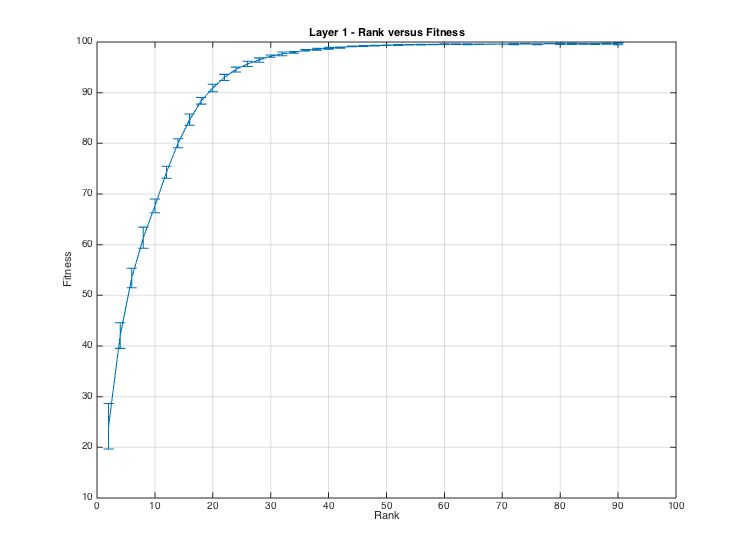
\includegraphics[width=\textwidth]{images/Layer1ImageNet.png}
    \caption{Conv Layer 1}
  \end{subfigure}
  \begin{subfigure}[h]{0.40\textwidth}
    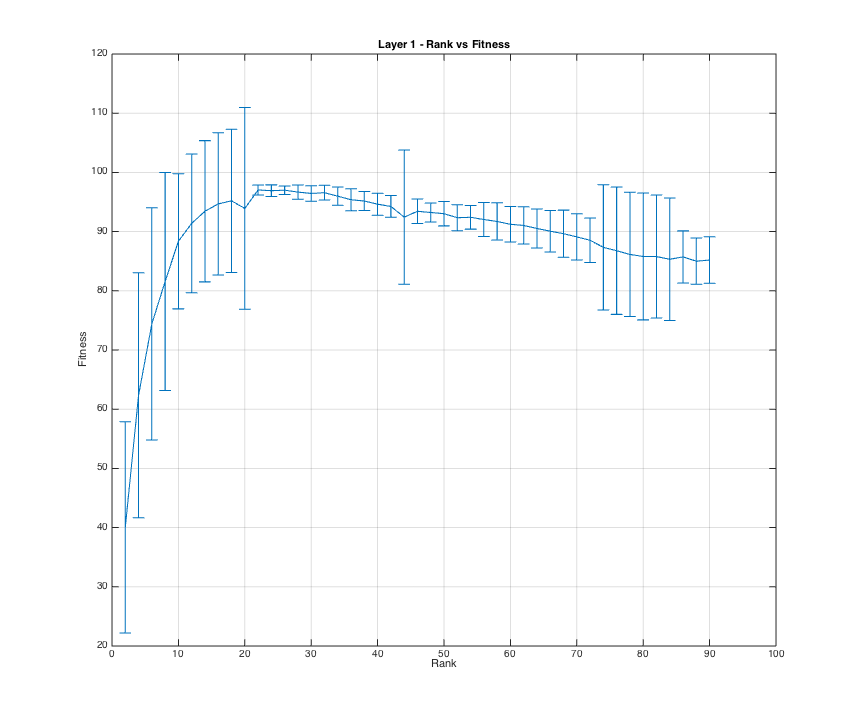
\includegraphics[width=\textwidth]{images/Layer2ImageNet.png}
    \caption{Conv Layer 2}
  \end{subfigure}
  \begin{subfigure}[h]{0.40\textwidth}
   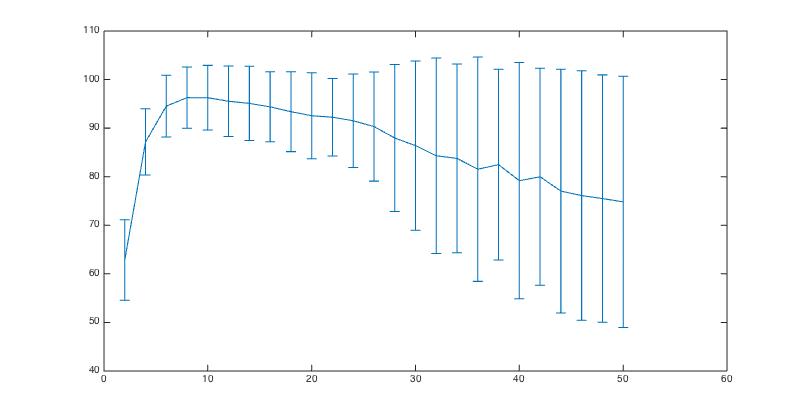
\includegraphics[width=\textwidth]{images/Layer3ImageNet.png}
    \caption{Conv Layer 3}
  \end{subfigure}
  \begin{subfigure}[h]{0.40\textwidth}
    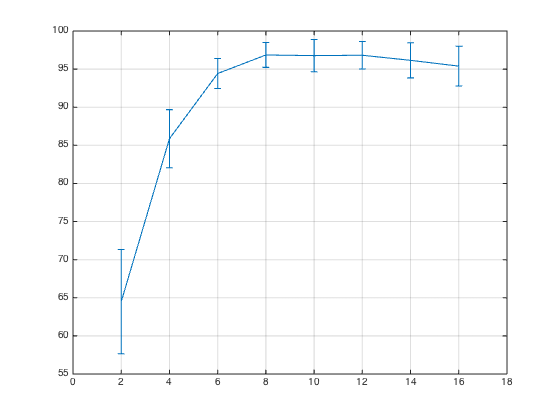
\includegraphics[width=\textwidth]{images/Layer4ImageNet.png}
    \caption{Conv Layer 4}
  \end{subfigure}
  \caption{Rank versus Fit for CNN Layers of ImageNet model. Conv L1 can have a theoretical 2 fold speedup while the approximation is almost perfect (rank aprox 45 with fit 99.9). For the following layers, the optimization algorithm starts to struggle and needs to be rerun multiple times. For a similar 2-fold speedup per layer, we would need to use a rank for which the fit is less than 90.}
  \label{fig:user_artiststribution}
\end{figure}